\documentclass[aspectratio=169]{beamer}
\usetheme{Uppsala}
\usepackage[caption=false]{subfig}
\usepackage[]{graphicx}
\usepackage{tikz}
\usepackage[]{physics}

\usetikzlibrary{arrows.meta}
\usetikzlibrary{decorations.pathreplacing}
\usetikzlibrary{decorations.markings}
\usetikzlibrary{patterns}
\usetikzlibrary{3d}
\usetikzlibrary{math}
\usetikzlibrary{calc}

\author[Ola Carlsson]{Ola Carlsson \\ Handledare: Erik
Sjöqvist \\ Ämnesgranskare: Patrik Thunström}
\title{Klassisk rörelse runt syntetiska
        magnetiska monopoler}
\subtitle{Kandidatarbete 15 hp}
\date[\today]{\today}
\institute[Institutionen för fysik och
astronomi]{Institutionen för fysik och astronomi,
Avdelningen för Materialteori}

\begin{document}
%% For the title
\begin{frame}[plain]
  \titlepage
\end{frame}
\begin{frame}
  \frametitle{Magnetiska monopoler}
  \begin{itemize}
          \item Magnetism liknar elektricitet, men är
                  inte samma sak.
          \item Ren magnetisk laddning finns inte
  \end{itemize}
\end{frame}
\begin{frame}
        \begin{figure}[h]
                \centering
                \subfloat[Electricity]{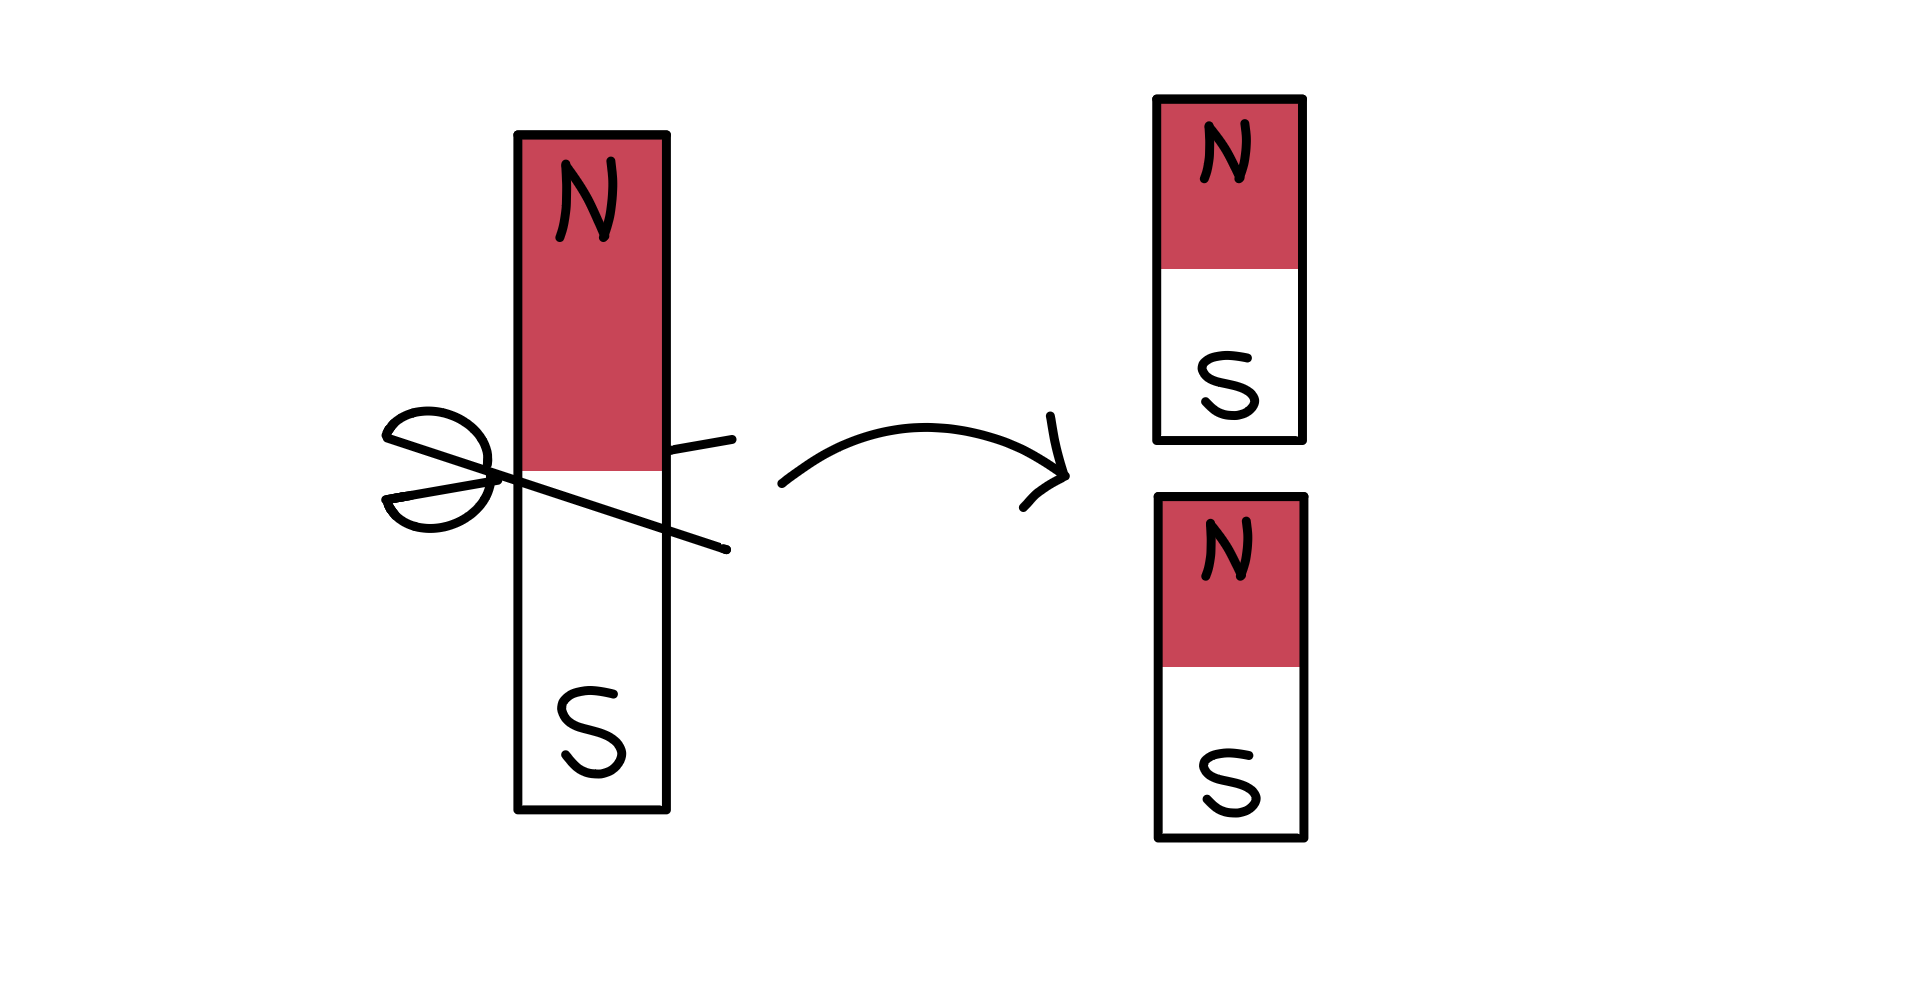
\includegraphics[width=0.5\textwidth]{magnetslice}}
                \subfloat[Magnetism]{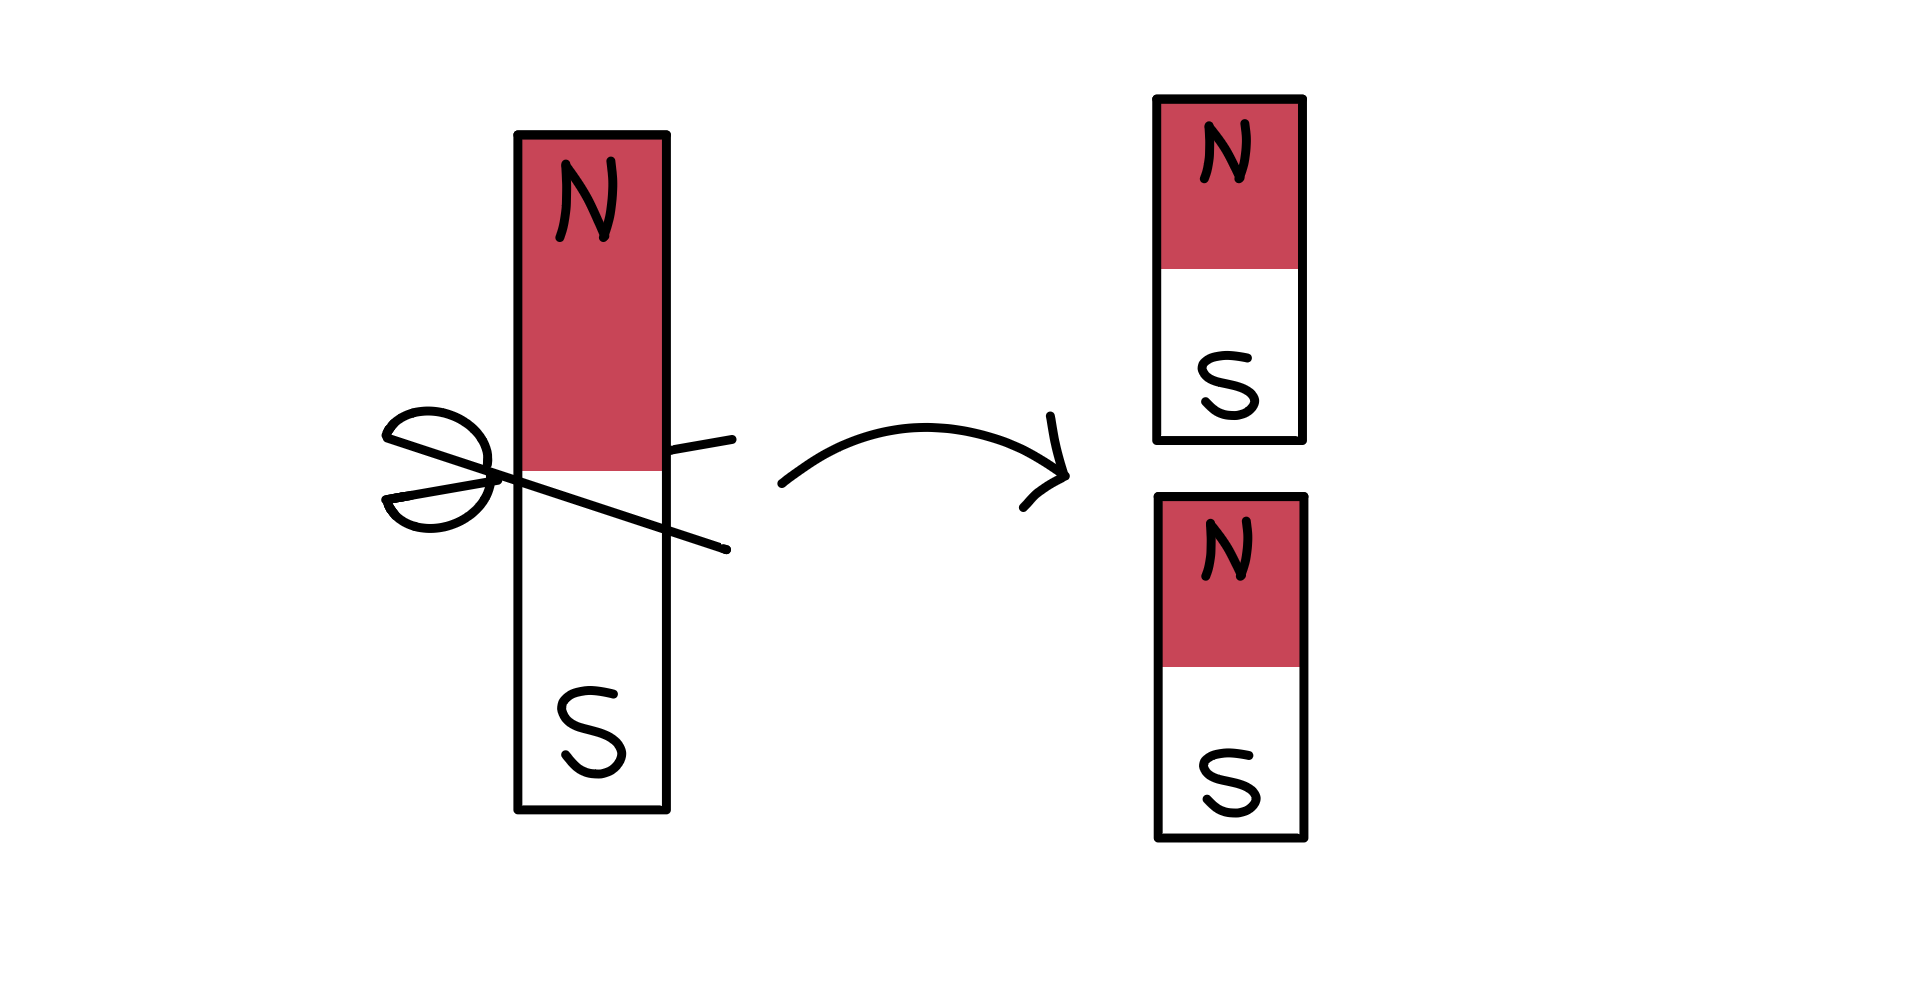
\includegraphics[width=0.5\textwidth]{magnetslice}}
        \end{figure}
\end{frame}
\begin{frame}
  \frametitle{Magnetiska monopoler}
  \begin{itemize}
          \item Magnetism liknar elektricitet, men är
                  inte samma sak.
          \item Ren magnetisk laddning finns inte.
          \item Sådan laddning vore 
                  "magnetiska monopoler".
          \item "Riktiga" magnetiska monopoler finns ej,
                  men monopolbeteende finns i naturen.
          \item Ett (obskyrt) exempel är "syntetiska"
                  monopoler som dyker upp vid
                  QM-approximationer.
  \end{itemize}
\end{frame}

\begin{frame}
        \frametitle{Syntetiska magnetiska monopoler}
        \begin{itemize}
                \item I vissa scenarion alstras ett
                        "syntetiskt fält" i
                        parameterrummet av monopoler.
                \item Det syntetiska fältet är
                        \textit{inte} ett vanligt
                        magnetfält, men det beter sig
                        väldigt mycket som ett.
                \item Det här projektet har modellerat
                        ett system som uppvisar
                        syntetiska monopoler, för att
                        undersöka mer precist hur de
                        påverkar världen.
        \end{itemize}
\end{frame}

\begin{frame}
        \frametitle{Hanteln}
        \begin{columns}
            \begin{column}{.49\textwidth}
                \begin{itemize}
                    \item Två massor som sitter fast på fixt
                        avstånd från varandra liknar en
                        hantel.
                    \item Var ände på hanteln är en dipol,
                        har spin.
                    \item Spin är som en stavmagnet som kan
                        rotera, fast på kvantmekaniskt
                        vis.
                    \item Hanteln blir då en slags
                        komplicerad magnet, som
                        påverkas av yttre
                        magnetfält.
                \end{itemize}
            \end{column}
            \begin{column}{.49\textwidth}
                \begin{figure}
        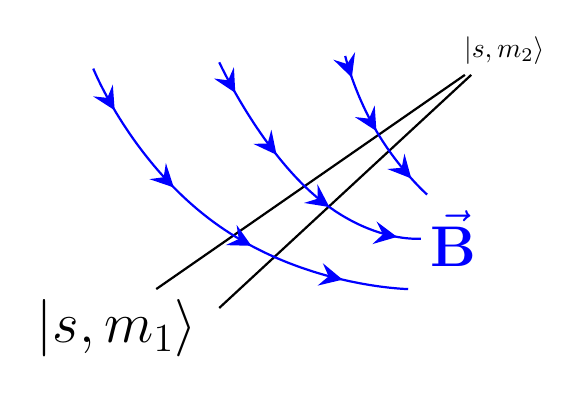
\begin{tikzpicture}[scale=0.8]
            \draw[black, thick] 
                    node[anchor=north,
                    xshift=-0.5cm]{\huge\(\ket{s, m_1}\)} (0,0) -- (4.9,3.4)
                    node[anchor=south, xshift=0.5cm]{\(\ket{s, m_2}\)};
            \draw[black, thick] (1, -0.3) -- (5,3.4);
            \draw[blue, thick, postaction=decorate, decoration={pre length = 1mm, post length = 1mm, markings, mark=
                        between positions 0.1 and 1 step
                        0.25 with {\pgftransformscale{2}\arrow{stealth}}}] plot [smooth, tension=1] coordinates {(-1,3.5) (1,1) (4,0)};
            \draw[blue, thick, postaction=decorate, decoration={pre length = 1mm, post length = 1mm, markings, mark=
                        between positions 0.1 and 1 step
                        0.4 with {\pgftransformscale{2}\arrow{stealth}}}] plot [smooth, tension=1] coordinates {(3,3.7) (3.5,2.5) (4.3,1.5)};
            \draw[blue, thick,  postaction=decorate, decoration={pre length = 1mm, post length = 1mm, markings, mark=
                        between positions 0.1 and 1 step
                        0.28 with {\pgftransformscale{2}\arrow{stealth}}}] plot [smooth, tension=1] coordinates {(1,3.6) (2.5,1.5) (4.2,0.8)};
            \draw[blue] (4.2,0.8) node[anchor=west, xshift=0cm]{\huge\(\va{B}\) };
        \end{tikzpicture}
                \end{figure}
 %\includegraphics[\textwidth]{fig}
 \end{column}
\end{columns}
\end{frame}

\begin{frame}
        \frametitle{Hanteln genom ett magnetfält}
        \begin{columns}
                \begin{column}{0.49\textwidth}
        \begin{itemize}
                \item Exakt hur rör sig hanteln genom
                        ett yttre magnetfält från säg
                        två spolar?
                \item Många komplicerande
                        omständigheter, men
                        Born-Oppenheimer-approximationen
                        löser problemet.
                \item Med B-O dyker de syntetiska fälten
                        och monopolerna upp.
                \item Rörelseekvationer hittades och
                        systemet simulerades m.h.a.
                        skript.
        \end{itemize}
        \end{column}
        \begin{column}{0.49\textwidth}
        \begin{figure}[h]
                \centering
                \def\dgrid[####1](####2,####3)(####4)(####5)(####6){ %[draw options](corner)(distance in x)
                %(distance in y)(number of lines -1  per side)
                \foreach \x in {0,1,...,####6}{
                        \pgfmathsetmacro\sx{\x*####4/####6}
                        \draw[####1] (####2+\sx,####3) -- (####2+\sx,####3+####5);
                        }
                \foreach \y in {0,1,...,####6}{
                        \pgfmathsetmacro\sy{\y*####5/####6}
                        \draw[####1] (####2,####3+\sy) -- (####2+####4, ####3+\sy);
                        }
                }
                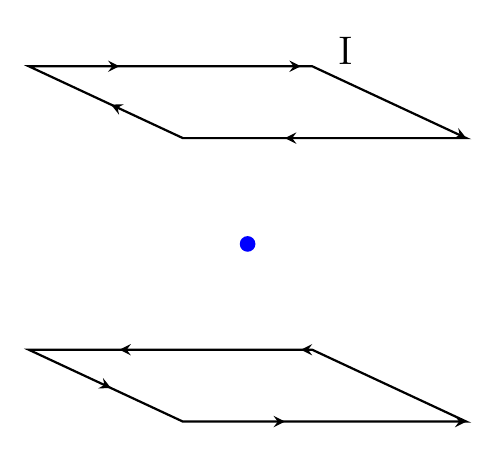
\begin{tikzpicture}[decoration={markings, mark= between positions 0.1 and 1 step
                        0.2 with {\arrow{stealth}}},
                        z={(90:10mm)},x={(-25:6mm)},y={(0:10mm)},
                        scale=0.6]
                    \begin{scope}[canvas is xy plane at z=0]
                        \draw[black, thick, postaction={decorate}] (0,0) -- (6,0) -- (6,6) -- (0,6) -- cycle;
                    \end{scope}
                    \dgrid[red, dotted, thick, canvas is xy plane at z=1](1,1)(4)(4)(8); %Draw the lab
                    \dgrid[red, dotted, thick, canvas is xy plane at z=5](1,1)(4)(4)(8);
                    \dgrid[red, dotted, thick, canvas is yz plane at x=1](1,1)(4)(4)(8);
                    \draw[blue] (3,3,3) node[circle, fill, inner sep=2pt]{}; %Zerofield marker
                    \dgrid[red, dotted, thick, canvas is yz plane at x=5](1,1)(4)(4)(8);
                    \dgrid[red, dotted, thick, canvas is zx plane at y=1](1,1)(4)(4)(8);
                    \dgrid[red, dotted, thick, canvas is zx plane at y=5](1,1)(4)(4)(8);
                    \begin{scope}[canvas is xy plane at z=6]
                        \draw[black, thick, postaction={decorate}] (0,0) -- (0,6)
                                node[anchor=west, xshift=2mm, yshift=2mm]{\Large I} -- (6,6) -- (6,0) -- cycle;
                    \end{scope}
                \end{tikzpicture}
        \end{figure}
        \end{column}
        \end{columns}
\end{frame}
\begin{frame}
        \frametitle{Simulationer}
    \begin{figure}[h]
        \centering
        \subfloat[\centering \(n =
        0\)]{{\includegraphics[width=3cm]{figures/n_compare/I10nr101lablength0.001tmax0.1J100000.0Gamma10000000000.0mass3.58e-25len5e-05n0vel(0.01,
                0, 0, 0, 0)swarmnum4norotFalsenosynFalse}}}
        \qquad
        \subfloat[\centering \(n = 1\)]{{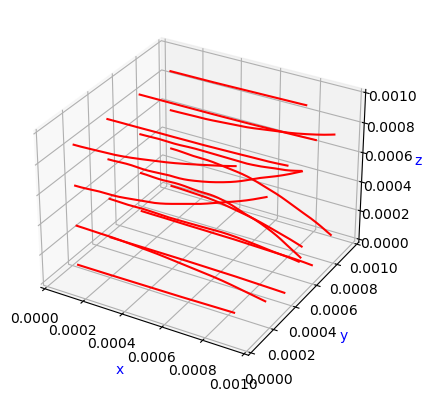
\includegraphics[width=3cm]{figures/n_compare/I10nr101lablength0.001tmax0.1J100000.0Gamma10000000000.0mass3.58e-25len5e-05n1vel(0.01, 0, 0, 0, 0)swarmnum4norotFalsenosynFalse}}}
        \qquad
        \subfloat[\centering \(n = 2\)]{{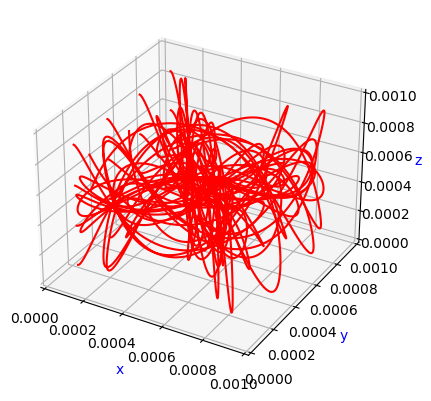
\includegraphics[width=3cm]{figures/n_compare/I10nr101lablength0.001tmax0.1J100000.0Gamma10000000000.0mass3.58e-25len5e-05n2vel(0.01, 0, 0, 0, 0)swarmnum4norotFalsenosynFalse}}}
    \end{figure}
    \begin{itemize}
            \item Banor för olika s.k. egentillstånd
                    ovan. Den höga energin längst till
                    höger är mest intressant.
    \end{itemize}
\end{frame}

\begin{frame}
        \frametitle{Simulationer}
    \begin{figure}[h]
        \centering
        \subfloat[\centering
        ''Stor'' massa]{{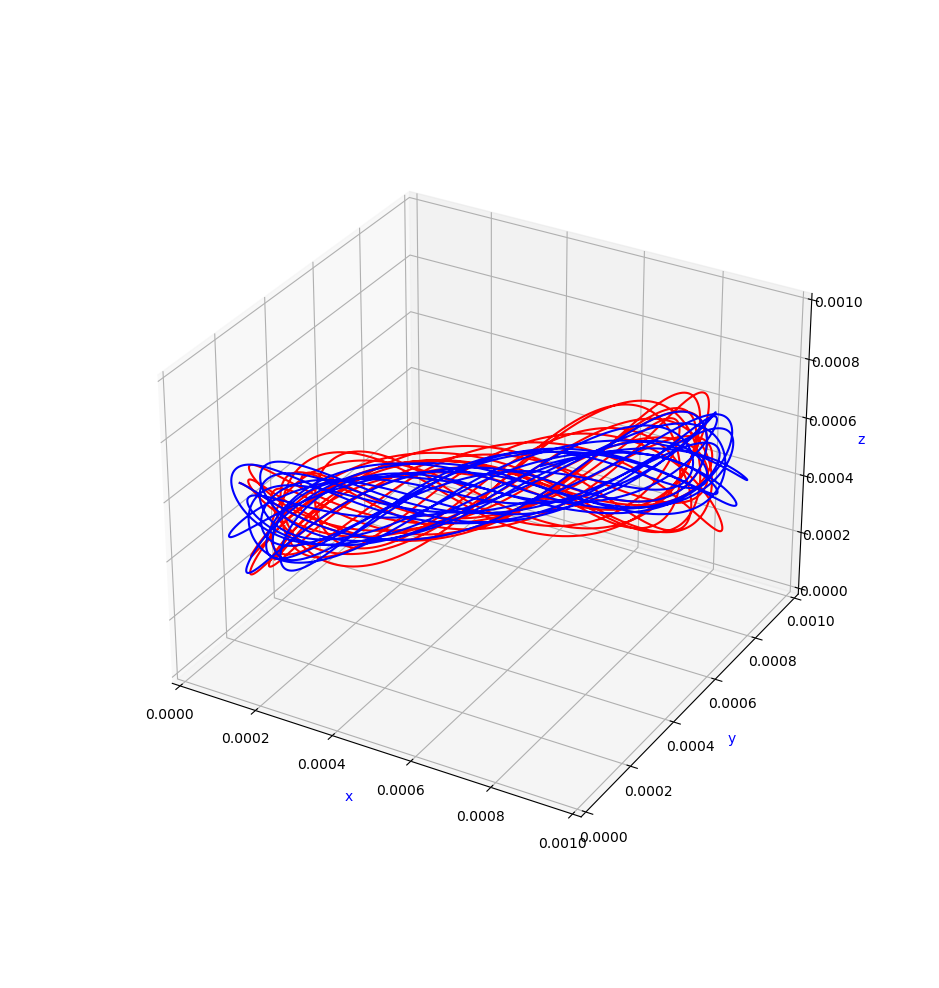
\includegraphics[width=4.5cm]{figures/n2m-25/(0,2)-comp1}}}
        \qquad  
        \subfloat[\centering
        ''Liten'', men rimlig, massa]{{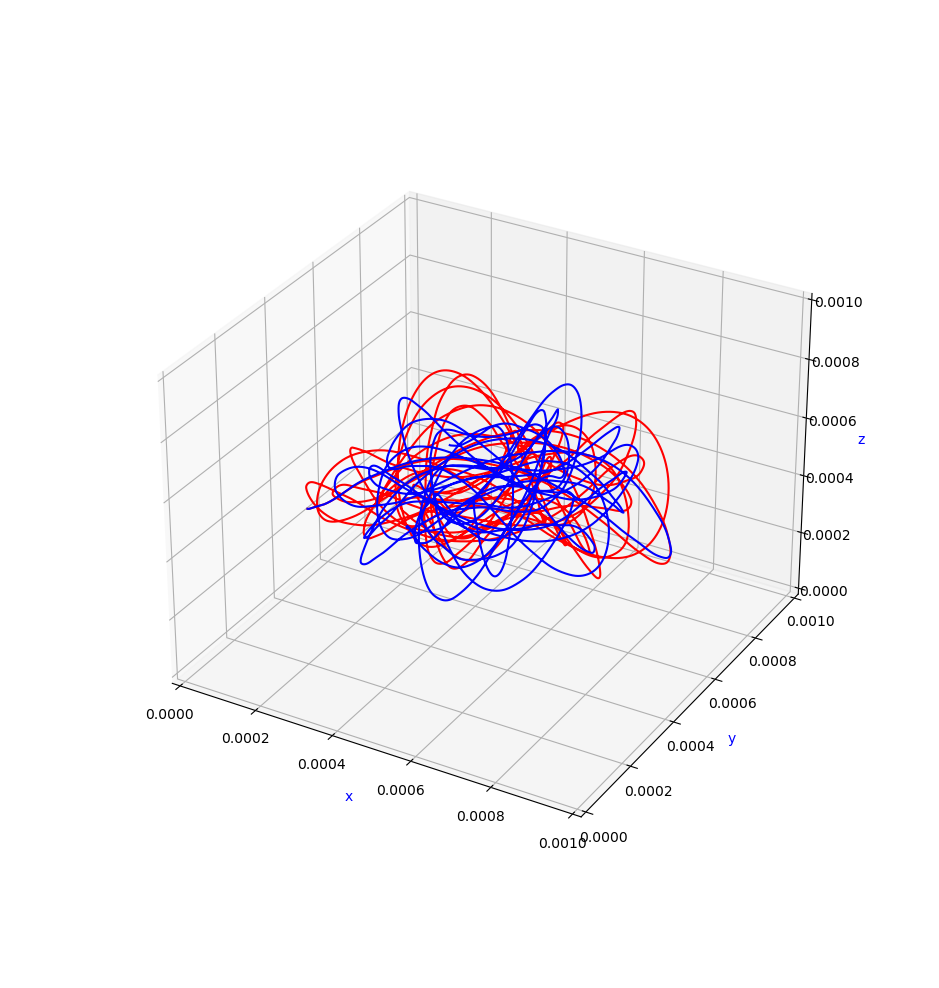
\includegraphics[width=4.5cm]{figures/n2m-27/(1,1)-comp1}}}
    \end{figure}
    \begin{itemize}
            \item Banor för olika hantel-massor ovan. Med syntetiska fält i rött, utan syntetiska fält i blått.
    \end{itemize}
\end{frame}
\begin{frame}
        \frametitle{Vidare arbete}
        \begin{itemize}
                \item  Kan vi se att det är just
                        monopoler i kulisserna?
                \item Prestanda i koden begränsar,
                        optimera eller kör på bättre
                        hårdvara (UPPMAX).
                \item Kan ett experiment som realiserar
                        modellen konstrueras?
                        Massuppskattingen utesluter inte
                        något vätgasliknande.
        \end{itemize}
\end{frame}
\end{document}
